
%----------------------------------------------------------------------------------------------------------------------------------------

% définit le type de document et ses options
\documentclass[a4paper,10pt]{article}

% des paquetages indispensables, qui ajoutent des fonctionnalites
\usepackage[utf8]{inputenc}
\usepackage{graphicx}
\usepackage{lscape}
\usepackage{url}
\usepackage{xspace}
\usepackage[francais]{babel}
%\usepackage{fullpage}

\pagestyle{plain}


%----------------------------------------------------------------------------------------------------------------------------------------


% le debut du contenu
\begin{document}


%----------------------------------------------------------------------------------------------------------------------------------------


%%%%%%%%%%%%%%%%%%%%%%%%%%%%%%%%%%%%%%%%%%%%%%%%%
%%Page d'accueil
\begin{center}
	%%
	\hspace{3cm}
	
\includegraphics[scale=0.8]{logo.ps}

	%%
	\vspace{1cm}
	{\large Projet de spécialité 2010}\\
	{\Large Conception d'un modèle de feu 3D temps réel}\\
	\vspace{1cm}


	\includegraphics[scale=0.3]{feu.ps}\\
	\vspace{2cm}
	%%
	Etudiants impliqués :\\
	Benjamin Aupetit - IRVM - benjamin.aupetit@ensimag.imag.fr\\
	Julien Champeau - IRVM - julien.champeau@ensimag.imag.fr\\
	Arnaud Emilien - IRVM - arnaud.emilien@ensimag.imag.fr\\
	~\\
	Encadrants :\\
	Marie-Paule Cani  -  Marie-Paule.Cani@inrialpes.fr \\
	Aurélie Catel - aurelie.catel@grenoble-inp.fr
	~ \\
	\vspace{3mm}
	Ensimag 2010\\

\end{center}

\newpage

\tableofcontents

\newpage



%----------------------------------------------------------------------------------------------------------------------------------------
%%%%%%%%%%%%%%%%%
\section{Présentation du projet}
\subsection{Introduction}

\subsection{Objectifs}


\subsection{Aperçu}


\subsection{Analyses Bibliographiques}
%%%%%%%%%%%%%%%%%
Cette section regroupe les différents articles lus, concernant les travaux déjà effectués dans ce domaine. 
Nous allons expliquer brièvement de quoi ils parlent, ce que nous en avons retenu de bien ou de mal, ce que nous allons 
utiliser...

\subsubsection{Real-Time Fluid Dynamics for Games}
\textbf{Auteurs} : Jos Stam.\\

\textbf{Publication} : Proceedings of the Game Developer Conference, March 2003 \\

\textbf{Sujet(s) abordé(s)} : \\Modèle de fluide temps réel, pouvant être utilisé pour le feu, la fumée\\
	Le modèle gère: le deplacement du fluide, la gestion de combustible,les forces appliquées sur le fluide.\\
	
\textbf{Principe} :\\
	Le modèle a été décomposé sur plusieurs étapes : génération du fluide par des sources, ajout des forces, diffusion du 		fluide, puis résolution de l'équation de la densité et de l'équation de la vitesse (équations de Navier-Stockes).
	Pour résoudre les deux équations, il utilise une astuce permettant de résoudre le système très rapidement.
	Enfin, il utilise le principe de conservation de la masse, qui rajoute des effets réalistes de vortex, avec la 		décomposition de Hodge.\\


\textbf{Point(s) positif(s)} :\\
	C'est facile à implémenter (moins de 100 lignes pour la version 2D)\\
	Peut être adapté pour la propagation du feu.\\
	Peut être adapté pour qu'un objet influe sur le modèle.\\
	Résultat réellement joli et réaliste.\\
	Très bien expliqué.\\
	Il a fournit un exemple 2D pour de la fumée, plutôt impréssionant.\\

\textbf{Point(s) négatif(s)} :\\
	La zone d'influence est assez petite, il faut voir si c'est possible de l'étendre sans trop allourdir les calculs. (Octree?) \\
	Pas trop de détails sur la représentation graphique du feu.\\
	
\textbf{Conclusion} :\\
	C'est sans doute ce que nous allons adapter, pour qu'il serve à la fois pour le feu, la fumée, et la propagation.

\subsubsection{Stable Fluids}
\textbf{Auteurs} : Jos Stam.\\
\textbf{Publication} : SIGGRAPH 99 Conference Proceedings\\
\textbf{Sujet(s) abordé(s)} : Résolution de l'équation des fluides ( Navier-Stockes) avec un algorithme stable.\\
\textbf{Point(s) positif(s)} :\\
\textbf{Point(s) négatif(s)} :\\
\textbf{Conclusion} :\\


\subsubsection{An Interactive Simulation Framework for Burning Objets}
\textbf{Auteurs} : Zeki Melek, John Keyser.\\
\textbf{Publication} :\\
\textbf{Sujet(s) abordé(s)} : \\
\textbf{Point(s) positif(s)} :\\
\textbf{Point(s) négatif(s)} :\\
\textbf{Conclusion} :\\


\subsubsection{Visual Simulation of Smoke}
\textbf{Auteurs} : Ronald Fedkiw, Jos Stam, Henrik Wann Jensen.\\
\textbf{Publication} :\\
\textbf{Sujet(s) abordé(s)} : \\
\textbf{Point(s) positif(s)} :\\
\textbf{Point(s) négatif(s)} :\\
\textbf{Conclusion} :\\

\subsubsection{Simulating Water and Smoke with an Octree Data Structure}
\textbf{Auteurs} : Frank Losasso, Frédéric Gibou, Ron Fedkiw.\\
\textbf{Publication} :\\
\textbf{Sujet(s) abordé(s)} : \\
\textbf{Point(s) positif(s)} :\\
\textbf{Point(s) négatif(s)} :\\
\textbf{Conclusion} :\\



\subsubsection{Real-Time Simulation of Deformation and Fracture of Stiff Materials}
\textbf{Auteurs} : Matthias Müller, Leonard McMillan, Julie Dorsey, Robert Jagnow.\\
\textbf{Publication} :\\
\textbf{Sujet(s) abordé(s)} : \\
\textbf{Point(s) positif(s)} :\\
\textbf{Point(s) négatif(s)} :\\
\textbf{Conclusion} :\\



\subsubsection{Voxels On Fire}
\textbf{Auteurs} : Ye Zhao, Xiaoming Wei, Zhe Fan, Arie Kaufman, Hong Qin.\\
\textbf{Publication} :\\
\textbf{Sujet(s) abordé(s)} : \\
\textbf{Point(s) positif(s)} :\\
\textbf{Point(s) négatif(s)} :\\
\textbf{Conclusion} :\\

\subsubsection{Meshes On Fire}
\textbf{Auteurs} : Haeyoung Lee, Laehyun, Mark Meyer, Mathieu Desbrun.\\
\textbf{Publication} :\\
\textbf{Sujet(s) abordé(s)} : Propagation des flammes à la surface d'un objet.\\
\textbf{Point(s) positif(s)} :\\
\textbf{Point(s) négatif(s)} :\\
\textbf{Conclusion} :\\

\subsubsection{Real-time Procedural Volumetric Fire}
\textbf{Auteurs} : Alfred R. Fuller, Hari Krishnan, Karim Mahrous, Bernd Hamann, Kenneth I. Joy.\\
\textbf{Publication} :\\
\textbf{Sujet(s) abordé(s)} : \\
\textbf{Point(s) positif(s)} :\\
\textbf{Point(s) négatif(s)} :\\
\textbf{Conclusion} :\\



%----------------------------------------------------------------------------------------------------------------------------------------
%%%%%%%%%%%%%%%%%
\section{Mise en place du modèle global}
%%%%%%%%%%%%%%%%%




%----------------------------------------------------------------------------------------------------------------------------------------
%%%%%%%%%%%%%%%%%
\section{Modèle de flamme}
%%%%%%%%%%%%%%%%%





%----------------------------------------------------------------------------------------------------------------------------------------
%%%%%%%%%%%%%%%%%
\section{Modèle de fumée}
%%%%%%%%%%%%%%%%%





%----------------------------------------------------------------------------------------------------------------------------------------
%%%%%%%%%%%%%%%%%
\section{Propagation sur l'objet}
%%%%%%%%%%%%%%%%%





%----------------------------------------------------------------------------------------------------------------------------------------
%%%%%%%%%%%%%%%%%
\section{Destruction de l'objet}
%%%%%%%%%%%%%%%%%





%----------------------------------------------------------------------------------------------------------------------------------------
%%%%%%%%%%%%%%%%%
\section{Propagation dans l'environnement}
%%%%%%%%%%%%%%%%%


%----------------------------------------------------------------------------------------------------------------------------------------
%%%%%%%%%%%%%%%%%
\section{Références}
%%%%%%%%%%%%%%%%%


%----------------------------------------------------------------------------------------------------------------------------------------
\end{document}
